%%%%%%%%%%%%%%%%%%%%%%%%%%%%%%%%%%%%%%%%%
% Programming/Coding Assignment
% LaTeX Template
%
% This template has been downloaded from:
% http://www.latextemplates.com
%
% Original author:
% Ted Pavlic (http://www.tedpavlic.com)
%
% Note:
% The \lipsum[#] commands throughout this template generate dummy text
% to fill the template out. These commands should all be removed when 
% writing assignment content.
%
% This template uses a Perl script as an example snippet of code, most other
% languages are also usable. Configure them in the "CODE INCLUSION 
% CONFIGURATION" section.
%
%%%%%%%%%%%%%%%%%%%%%%%%%%%%%%%%%%%%%%%%%

%----------------------------------------------------------------------------------------
%	PACKAGES AND OTHER DOCUMENT CONFIGURATIONS
%----------------------------------------------------------------------------------------

\documentclass{article}
\usepackage{fancyhdr} % Required for custom headers
\usepackage{lastpage} % Required to determine the last page for the footer
\usepackage{extramarks} % Required for headers and footers
\usepackage[usenames,dvipsnames]{color} % Required for custom colors
\usepackage{graphicx} % Required to insert images
\usepackage{caption}
\usepackage{listings} % Required for insertion of code
\usepackage{courier} % Required for the courier font
\usepackage{lipsum} % Used for inserting dummy 'Lorem ipsum' text into the template
\usepackage[colorlinks=true,linkcolor=black,anchorcolor=black,citecolor=black,menucolor=black,runcolor=black,urlcolor=black,bookmarks=true]{hyperref}
\usepackage[table,svgnames]{xcolor}
\usepackage{tabularx}
\usepackage{booktabs}
\usepackage{natbib}

% Margins
\topmargin=-0.45in
\evensidemargin=0in
\oddsidemargin=0in
\textwidth=6.5in
\textheight=9.0in
\headsep=0.25in

\linespread{1.1} % Line spacing

% Set up the header and footer
\pagestyle{fancy}
\lhead{\hmwkAuthorName} % Top left header
\chead{\hmwkClass\ (\hmwkClassInstructor\ \hmwkClassTime): \hmwkTitle} % Top center head
\rhead{\firstxmark} % Top right header
\lfoot{\lastxmark} % Bottom left footer
\cfoot{} % Bottom center footer
\rfoot{Page\ \thepage\ of\ \protect\pageref{LastPage}} % Bottom right footer
\renewcommand\headrulewidth{0.4pt} % Size of the header rule
\renewcommand\footrulewidth{0.4pt} % Size of the footer rule

\setlength\parindent{0pt} % Removes all indentation from paragraphs

%----------------------------------------------------------------------------------------
%	CODE INCLUSION CONFIGURATION
%----------------------------------------------------------------------------------------

\definecolor{MyDarkGreen}{rgb}{0.0,0.4,0.0} % This is the color used for comments
\lstloadlanguages{Perl} % Load Perl syntax for listings, for a list of other languages supported see: ftp://ftp.tex.ac.uk/tex-archive/macros/latex/contrib/listings/listings.pdf
\lstset{language=Perl, % Use Perl in this example
        frame=single, % Single frame around code
        basicstyle=\small\ttfamily, % Use small true type font
        keywordstyle=[1]\color{Blue}\bf, % Perl functions bold and blue
        keywordstyle=[2]\color{Purple}, % Perl function arguments purple
        keywordstyle=[3]\color{Blue}\underbar, % Custom functions underlined and blue
        identifierstyle=, % Nothing special about identifiers                                         
        commentstyle=\usefont{T1}{pcr}{m}{sl}\color{MyDarkGreen}\small, % Comments small dark green courier font
        stringstyle=\color{Purple}, % Strings are purple
        showstringspaces=false, % Don't put marks in string spaces
        tabsize=5, % 5 spaces per tab
        %
        % Put standard Perl functions not included in the default language here
        morekeywords={rand},
        %
        % Put Perl function parameters here
        morekeywords=[2]{on, off, interp},
        %
        % Put user defined functions here
        morekeywords=[3]{test},
       	%
        morecomment=[l][\color{Blue}]{...}, % Line continuation (...) like blue comment
        numbers=left, % Line numbers on left
        firstnumber=1, % Line numbers start with line 1
        numberstyle=\tiny\color{Blue}, % Line numbers are blue and small
        stepnumber=5 % Line numbers go in steps of 5
}

% Creates a new command to include a perl script, the first parameter is the filename of the script (without .pl), the second parameter is the caption




%----------------------------------------------------------------------------------------
%	DOCUMENT STRUCTURE COMMANDS
%	Skip this unless you know what you're doing
%----------------------------------------------------------------------------------------

% Header and footer for when a page split occurs within a problem environment
\newcommand{\enterProblemHeader}[1]{
\nobreak\extramarks{#1}{#1 continued on next page\ldots}\nobreak
\nobreak\extramarks{#1 (continued)}{#1 continued on next page\ldots}\nobreak
}

% Header and footer for when a page split occurs between problem environments
\newcommand{\exitProblemHeader}[1]{
\nobreak\extramarks{#1 (continued)}{#1 continued on next page\ldots}\nobreak
\nobreak\extramarks{#1}{}\nobreak
}

\setcounter{secnumdepth}{0} % Removes default section numbers
\newcounter{homeworkProblemCounter} % Creates a counter to keep track of the number of problems

\newcommand{\homeworkProblemName}{}
\newenvironment{homeworkProblem}[1][Problem \arabic{homeworkProblemCounter}]{ % Makes a new environment called homeworkProblem which takes 1 argument (custom name) but the default is "Problem #"
\stepcounter{homeworkProblemCounter} % Increase counter for number of problems
\renewcommand{\homeworkProblemName}{#1} % Assign \homeworkProblemName the name of the problem
\section{\homeworkProblemName} % Make a section in the document with the custom problem count
\enterProblemHeader{\homeworkProblemName} % Header and footer within the environment
}{
\exitProblemHeader{\homeworkProblemName} % Header and footer after the environment
}

\newcommand{\problemAnswer}[1]{ % Defines the problem answer command with the content as the only argument
\noindent\framebox[\columnwidth][c]{\begin{minipage}{0.98\columnwidth}#1\end{minipage}} % Makes the box around the problem answer and puts the content inside
}

\newcommand{\homeworkSectionName}{}
\newenvironment{homeworkSection}[1]{ % New environment for sections within homework problems, takes 1 argument - the name of the section
\renewcommand{\homeworkSectionName}{#1} % Assign \homeworkSectionName to the name of the section from the environment argument
\subsection{\homeworkSectionName} % Make a subsection with the custom name of the subsection
\enterProblemHeader{\homeworkProblemName\ [\homeworkSectionName]} % Header and footer within the environment
}{
\enterProblemHeader{\homeworkProblemName} % Header and footer after the environment
}

%----------------------------------------------------------------------------------------
%	NAME AND CLASS SECTION
%----------------------------------------------------------------------------------------

\newcommand{\hmwkTitle}{A4} % Assignment title
\newcommand{\hmwkDueDate}{Thursday,\ March\ 02,\ 2017} % Due date
\newcommand{\hmwkClass}{\ INTRO. TO WEB SCIENCE:\ CS 532} % Course/class
\newcommand{\hmwkClassTime}{} % Class/lecture time
\newcommand{\hmwkClassInstructor}{Dr. Nelson} % Teacher/lecturer
\newcommand{\hmwkAuthorName}{Udochukwu Nweke} % Your name

%----------------------------------------------------------------------------------------
%	TITLE PAGE
%----------------------------------------------------------------------------------------

\title{
\vspace{2in}
\textmd{\textbf{\hmwkClass:\ \hmwkTitle}}\\
\normalsize\vspace{0.1in}\small{Due\ on\ \hmwkDueDate}\\
\vspace{0.1in}\large{\textit{\hmwkClassInstructor\ \hmwkClassTime}}
\vspace{3in}
}

\author{\textbf{\hmwkAuthorName}}
\date{} % Insert date here if you want it to appear below your name

%----------------------------------------------------------------------------------------

\begin{document}

\maketitle

%----------------------------------------------------------------------------------------
%	TABLE OF CONTENTS
%----------------------------------------------------------------------------------------

%\setcounter{tocdepth}{1} % Uncomment this line if you don't want subsections listed in the ToC

\newpage
\tableofcontents
\newpage

%----------------------------------------------------------------------------------------
%	PROBLEM 1
%----------------------------------------------------------------------------------------

% To have just one problem per page, simply put a \clearpage after each problem

\begin{homeworkProblem}

Determine if the friendship paradox holds for my Facebook
account.* Compute the mean, standard deviation, and median of the
number of friends that my friends have.  Create a graph of the
number of friends (y-axis) and the friends themselves, sorted by
number of friends (x-axis).  (The friends don't need to be labeled
on the x-axis: just f1, f2, f3, ... fn.)  Do include me in the graph
and label me accordingly.


\lstinputlisting[caption=Extract Facebook Friend Count Code, language=python]{P1.py}
\lstinputlisting[caption=R Script to plot Friend Count. Calculate SD and Mean and Median of Friend Count, language=python]{P1.r}
\textbf{Solution 1:}

\begin{figure}
  \caption{Dr. Nelson's Friends vs Number of Friends}
  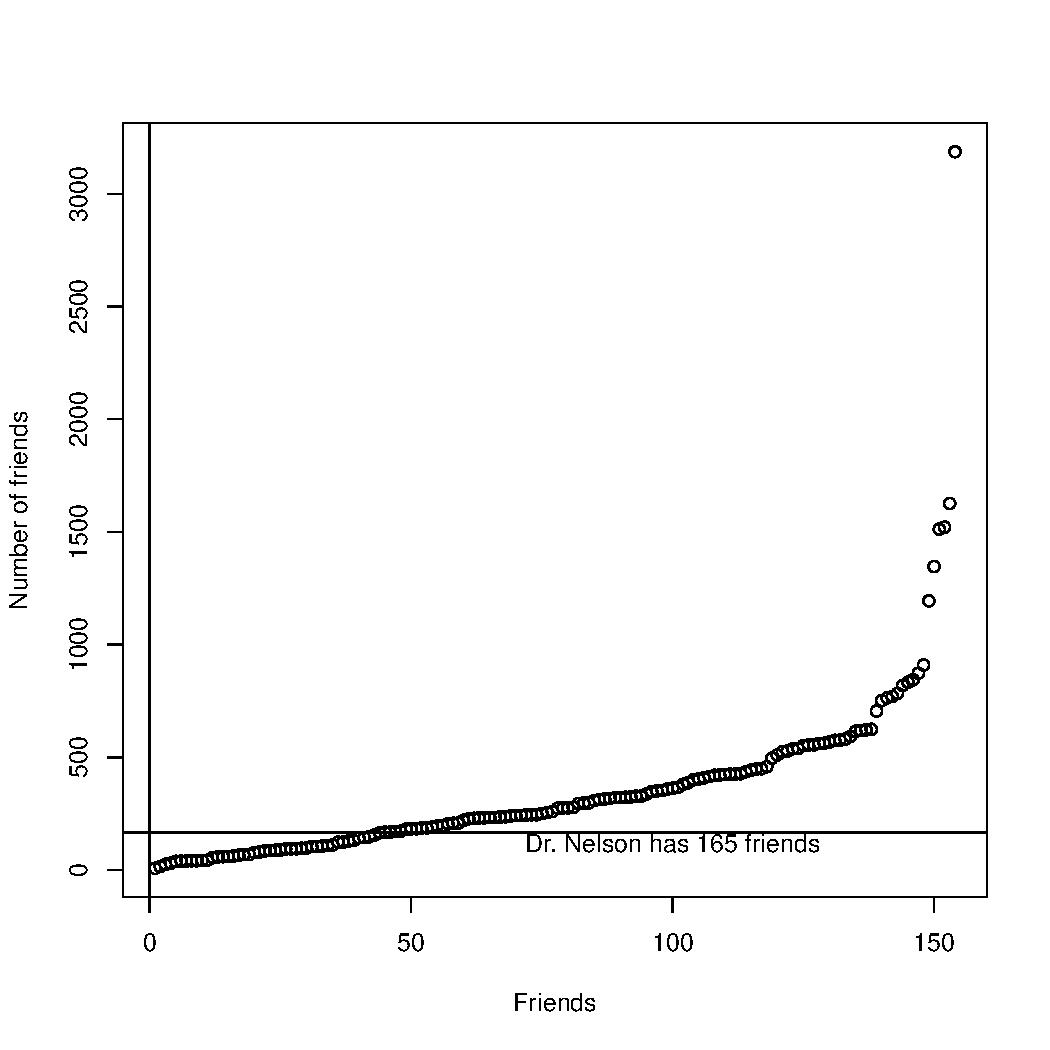
\includegraphics{Rplots}
\end{figure}

1. In order to get the names of Dr. Nelson's friend and their friends count, I used Beautiful soup to parse the given xml 
(mlnFriend.xml) into a structure. This is shown in listing 1, line 14- 15. \\

I wrote a dictionary \textit{getFriendCountDict} that generates the Friend and Friends counts and wrote the result into \textit{fb.mlnFriends.csv} file. This is seen in listing 1, and Table \ref{tab:nelsonFriendsSubset}\\

Dr. Nelson has a total number of 165 friends and 11 of his friends didn't have friend count. I called the 11 friends the problematic friends and skipped them in my \textit{fb.mlnFriends.csv} file record. \textit{nelsonFriendsStat.txt} contains the total number of freinds and number of problematic friends (Friends without friend count).

2. I wrote an R script to plot the friendship graph (Fig. 1) and compute the mean, median, and standard deviation. This is demonstrated in listing 2 line 1-5, and Table \ref{tab:Facebook Gragh}.

\begin{table}[h!]
   \centering
   \caption{Mean, median and SD numbers of Dr. Nelson's Facebook Friends}
    \label{tab:Facebook Gragh}
    \begin{tabular}{ | l | l | l|}
    \hline
   Mean &Median&Standard Deviation\\
   \hline
   359.0 &  266.5 & 371.5853 \\
   \hline
 \end{tabular}
\end{table}

Based on the graph and the statistics, Dr. Nelson has a total number of 154 friends. The mean and meadian number of his friends are 359.0 and 266.5 respectively. Therefore, the frienship paradox holds.

\begin{table}[h!]
 \centering
 \caption{Subset of Dr. Nelson's Facebook Friends and their respective Friends Count }
  \label{tab:nelsonFriendsSubset}
  \begin{tabular}{ | l | l | }
      \hline
     Friend &FriendsCount\\
     \hline
     Doug Nelson & 7  \\
     \hline
     Brian K. Saunders & 15\\
     \hline
     Winnie Elliott &25 \\
     \hline
     Joan A. Smith &30 \\
     \hline
     Bob Mathers &38 \\
     \hline
     Thomas Allen &39\\
     \hline
     Lloyd Nelson & 40\\
     \hline
     Scott W Laney & 41 \\
     \hline
     Mary McManus,&41 \\
     \hline
     Greg Szalkowski &42\\
     \hline
     Calvin Edward Mackey &1626\\
     \hline
     Ricardo Baeza-Yates & 3187\\
     \hline
  \end{tabular}
\end{table}

 \end{homeworkProblem}
%----------------------------------------------------------------------------------------
% PROBLEM 2
%----------------------------------------------------------------------------------------
\begin{homeworkProblem}

\lstinputlisting[caption=Retrieve Dr. Nelson's Twitter Followers Code, language=python]{P2.py}

\begin{table}[h!]
 \centering
 \caption{Subset of Dr Nelson's Twitter Friends and their respective Friends Count }
  \label{tab:alexa}
  \begin{tabular}{ | l | l | }
  \hline
 Friend &FriendsCount\\
 \hline
 KariHeffner & 4 \\
 \hline
 Past\_Pages & 5\\
 \hline
 ThoughtsFromBEL & 5 \\
 \hline
 normeu & 5 \\
 \hline
 involutish & 5 \\
 \hline
 karensnet & 5\\
 \hline
 awptix & 5\\
 \hline
 DanMilanko & 7 \\
 \hline
 SimpleSimon2013 & 9 \\
 \hline
 AmberBoehnlein& 9\\
 \hline
 neiltyson & 6829297\\
 \hline
 UberFacts & 13388960\\
 \hline

  \end{tabular}
\end{table}

  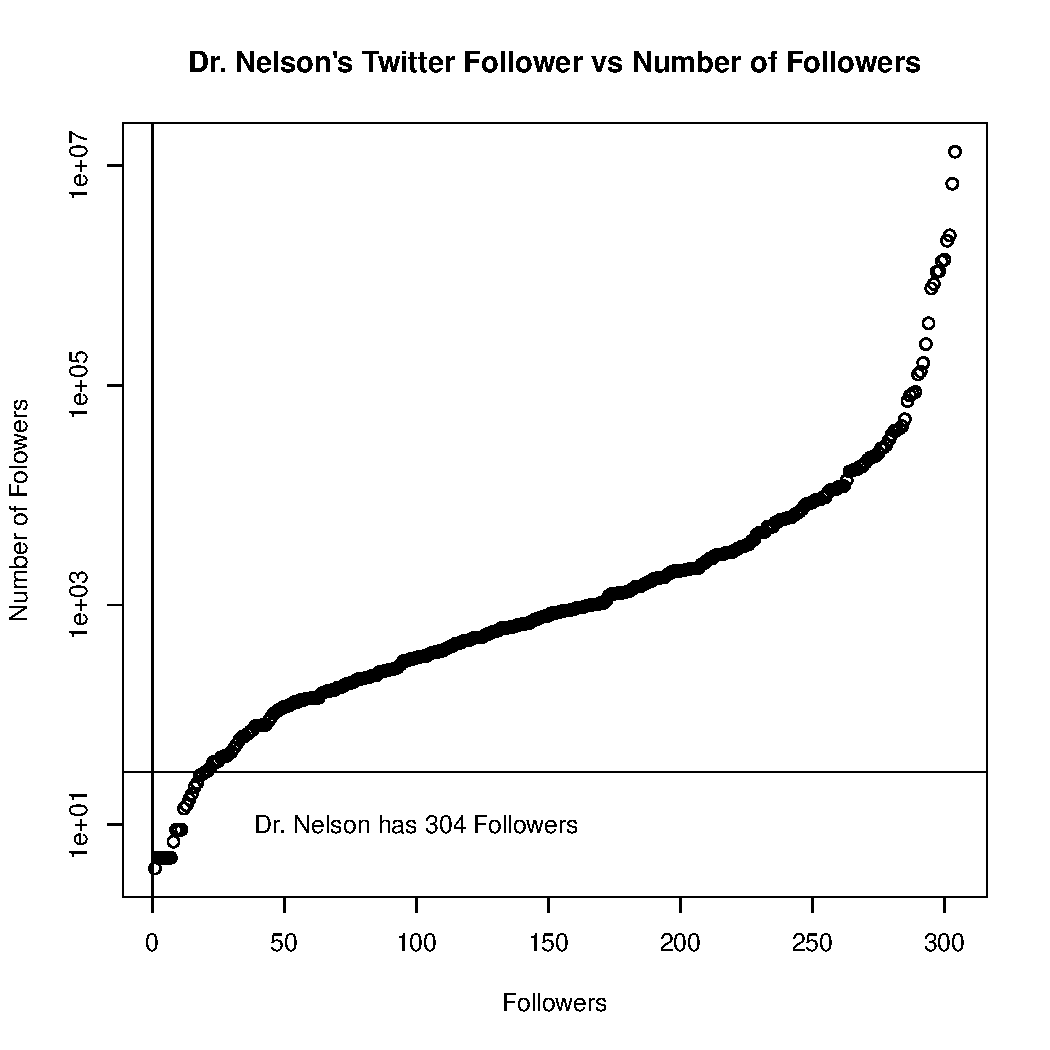
\includegraphics{TRplots}

2.  Determine if the friendship paradox holds for your Twitter account.
Since Twitter is a directed graph, use ``followers'' as value you measure
(i.e., ``do your followers have more followers than you?'').

  Generate the same graph as in question 1 and calcuate the same 
mean, standard deviation, and median values.

For the Twitter 1.1 API to help gather this data, see:

\url{https://dev.twitter.com/docs/api/1.1/get/followers/list}\\

\textbf{Solution 2:}\\

1. In other to retrieve Dr. Nelson's followers, I used Dr. Nelson's Twitter (phonedude\_mln) account and used a Twitter api wrapper-Tweepy to extract his followers. The function \textit{getFriendsDict} retrieves all Dr. Nelson's followers. This is demostrated in listing 3.\\

2. After getting the number of friends with \textit{getFriendsDict} function, I used \textit{writeFollowers} function the get Dr. Nelson's followers' count (friend count). This is shown in listing 3.

Table 2 contains a subset of Dr. Nelson's friend and their respective friends count. The complete list of Dr. Nelson's friends and their respective friends count is written in \textit{twitter.mlnFriends.csv}

I wrote an R script to generate the graph as outline in Listing 2, line 10-14.\\

\begin{table}[h!]
 \centering
 \caption{Mean, median and SD numbers of Dr. Nelson's Twitter Friends}
  \label{tab:Twitter Graph}
  \begin{tabular}{ | l | l | l|}
  \hline
 Mean &Median&Standard Deviation\\
 \hline
 110300 & 847 & 889156.8 \\
 \hline

 \end{tabular}
  \end{table}

Based on the graph and the statistics Table \ref{tab:Twitter Graph}, Dr. Nelson has 304 friends on twitter, but the mean and median of his friends are 110300 and 847 respectively. Hence, the friendship paradox holds.
 

\end{homeworkProblem}

\nocite{*}
\bibliographystyle{plain}
\bibliography{A4Ref}

\end{document}